%CHR started 17 Feb 2020, reproduction achieved 20 Feb 2020

%Notes for my submission to the 20-year reproducibility challenge by Konrad Hinsen and colleagues (https://rescience.github.io/ten-years/)

\section{Introduction}

The chosen article from 1995\supercite{Robert1995} described a new method for calculating friction coefficients of large, flexible DNA-protein complexes, with the goal of helping infer their structural properties from light scattering or ultracentrifugation data. The present report describes my successful effort to reproduce the results presented in the article, and offers some thoughts on the easier and more difficult parts of the task.

About two meters of DNA is packaged into every human cell nucleus, and a major focus of cell biology is on how eukaryotic cells in general reconcile this degree of compaction with the need to access the genetic message of the DNA. The packaged form of DNA is called chromatin, and it is composed in essence of regions of relatively free DNA interspersed by other regions in which about two turns of the DNA double helix are wrapped neatly around proteins called histones; these globular regions are called nucleosomes. The degree of chromatin compaction is locally dynamic; such remodelling reflects different biological imperatives in the cell cycle and adaptation to different metabolic contexts\supercite{Tian2016}.

The article presents an approach to modelling biophysical hydrodynamics data for these large systems (schematicized in article Figure 1), which consists of decomposing the molecule into globular and chain regions (nucleosomes and free DNA, respectively), then replacing each chain region by a single, calculated hydrodynamic sphere before calculating the average frictional properties of the entire assembly using Kirkwood-Bloomfield modelling\supercite{Bloomfield1977} together with appropriate chain conformational statistics. This results in a marked reduction in the number of required frictional elements, and simultaneously reduces errors arising from common hydrodynamics approximations.

The approach was validated on test geometries and applied to realistic chromatin structural models obtained using a novel mathematical 3D model of the 30 nm chromatin fiber, defined as a function of structural parameters including the number of superhelical turns of each nucleosome and the helical twist of the DNA double helix. General features of this modelling were presented briefly in the appendix.

\section{Targets}

The targets for reproduction were the following.

\begin{itemize}

\item \textbf{Calculations on reference assemblies.} The original article figure 2 showed a test of the method presented in the article for predicting translational friction coefficients of a series of  reference assemblies, whose exact properties had been reported earlier. These assemblies had two shapes (lollipop and dumbbell), and their dimensions were chosen to approximate the dimensions of a nucleosome along with free ``linker" DNA.

\item \textbf{Hydrodynamic force analysis.} Article figure 3 compared the translational force calculated using the Kirkwood-Bloomfield bead approximation coupled with the new method, versus the exact force calculated by the Zimm approach \supercite{Zimm1980}, as a function of bead separation depending on the free DNA length in basepairs (bp).

\item \textbf{Dinucleosome wrapping calculations}. The original article's figure 4 showed the translational diffusion coefficient for a system consisting of two nucleosomes positioned on a 354 bp DNA template, calculated using the new method and plotted as a function of the number of superhelical turns. The calculations were compared to experimental results from light-scattering experiments on a similar system obtained at two different salt concentrations.

\item \textbf{Analyzing a three-nucleosome compaction process.} The original work also demonstrated, in figure 5 and a table of values, the potential of the new calculation method for comparing different models for DNA compaction. Sedimentation coefficients were calculated for all possible intermediates in a hypothetical saturation of a 624 bp DNA template with up to three positioned nucleosomes, and the distributions obtained for histone binding in a cooperative versus a non-cooperative (random assembly) process.

\end{itemize}

\section{Methods}

The calculations reported in the 1995 article were all performed with Mathematica version 2.2 on a 1992 Macintosh IIci (Motorola 68030 clocked at 25 MHz) running macOS 7.1. All Mathematica notebooks for the article remained accessible throughout the intervening years in my project file directories.

 The reproducibility tests were performed using two different versions of Mathematica (running on three different platforms):

\begin{itemize}

\item Mathematica version 5.2, released in 2005, was first used, running on a late-2018 13-inch Macbook (Intel core i7, 2.7 GHz) running macOS 10.14 (Mojave). Note that Mathematica 5.2 will no longer run on macOS $\ge$ 10.15 (Catalina) because it contains 32-bit code.

\item All code was also run using Mathematica version 12.0, released in 2019, running under Raspbian linux on a Raspberry Pi 3 model B+ and 4 model B.

\end{itemize}

The numerical results presented in the article had been preserved in the original notebooks. Although not targets of this comparison \textit{per se}, the article figures (as opposed to numerical notebook data) had been produced either from the original Mathematica Postscript followed by some figure compositing, or by exporting numerical data for input to Cricket Graph (if memory serves-- I can't read those figure files now.)

All original and modified software described here has been made publicly available as a directory ``rehydro" on Zenodo. In preparing for the reproduction trials, the original notebooks were automatically converted using Mathematica v5.2 to an ascii format. The 1995 notebooks generally contained additional code and results unrelated to the article or to the present tests; all relevant code for each target was saved with the root filename addition ``\_1995" in the subdirectory ``originals". Copies of these files, with added filename code ``\_repro", were then used for all reproduction attempts and modified as necessary in order to obtain results for comparison. The original library notebook ``s6.1\_1995.nb", modified as necessary to ``s6.1\_repro.nb", plus a notebook ``extra.nb" containing additional plotting functions, were stored as Mathematica 5.2 packages with the suffix ``.m", and the ``Get" command added to the top of the relevant notebooks to execute them.

\textbf{Running notes:} In order to run the ``\_repro" files, a symbolic link "ReScience" pointing to the rehydro code directory was first placed in Mathematica's default working directory (my home directory in this case). Also, for each target, in order to remove history-dependent effects, the kernel was restarted and all target notebook cells were evaluated (answering ``No" to the dialog proposing to evaluate initialization cells only).

\section{Results}

%\begin{enumerate}

%\item Figure 2:
\subsection{Calculations on reference assemblies (original Figure 2)}

The article's approach was validated by using it to calculate translational frictional coefficients for two series of reference assemblies (points connected by solid lines in the figure). These were compared to exact values (black circles in the figure) and to values calculated using an existing approximation method (dotted lines).

The original notebook
 %``Figure\ 2\ calculations.nb"
contained all the necessary code to calculate the friction coefficients of the reference assemblies as well as the numerical values plotted in the article. The friction coefficients calculated in this notebook were thus the targets for the reproduction.

For the present reproduction trials, the notebook executed without any errors or warnings. The calculated friction coefficients match those obtained in the original notebook, differing only in the default rounding (4 digits in the original notebook, 6 in the new notebook). A plot of the data made using Mathematica 12 is shown in Figure \ref{figure2} for comparison to Figure 2 in the original article. Friction coefficients in the sub-50 bp spacer range had been calculated separately and were not present in the original files.

\begin{figure}[H]
\centering
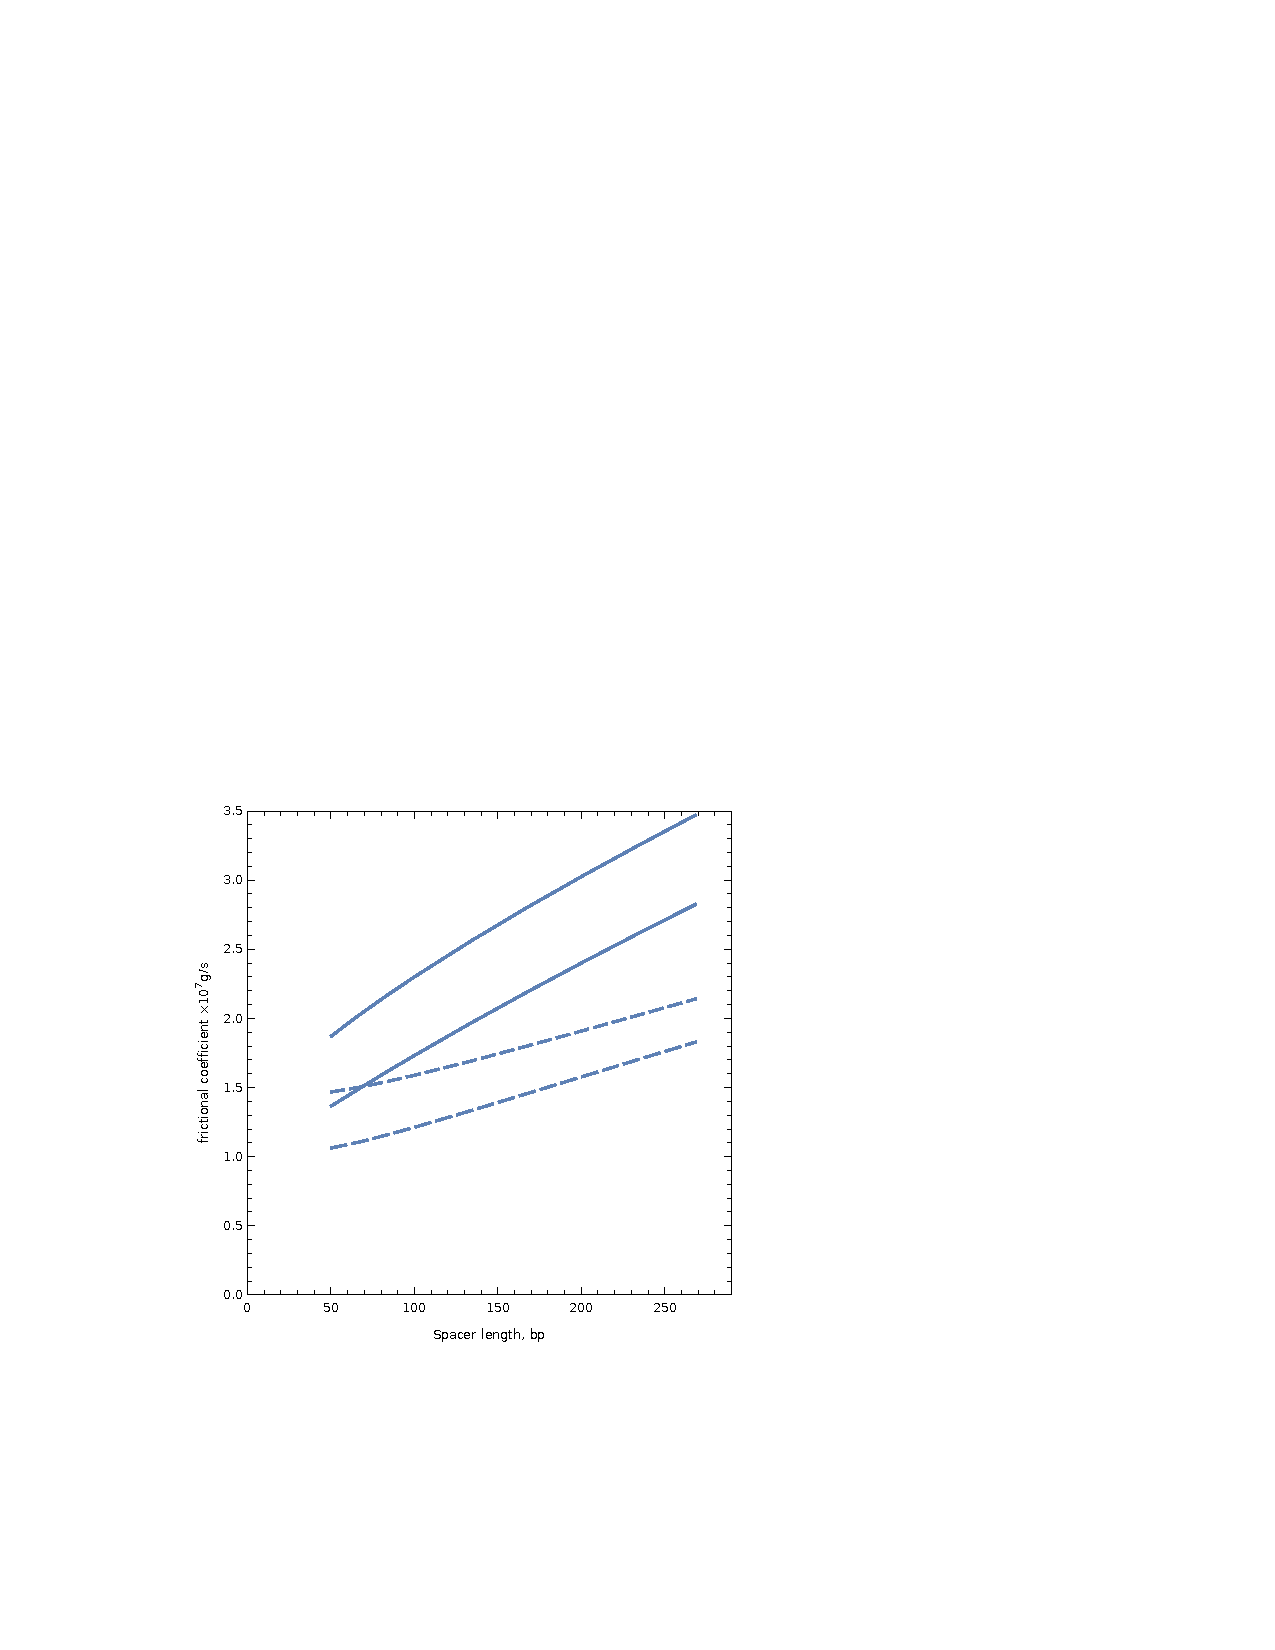
\includegraphics[width=0.5\textwidth]{figs/figure2M12.pdf}
\caption{Results of recalculation by Mathematica 12.0 of the translational friction coefficients for ``dumbbell" (upper curves) and ``lollipop" (lower curves) reference assemblies, for comparison to Figure 2 of the original article. Each assembly was calculated using the presented approach (solid line) and the standard approach (dashed line). The original figure also depicted corresponding ``exact" data points for reference, as calculated by other authors.}
\label{figure2}
\end{figure}


%\item Figure 3:
\subsection{Hydrodynamic force analysis (original Figure 3)}
An advantage of the presented approach was the elimination of contacting frictional elements, which otherwise led to errors in commonly used hydrodynamic force calculations. Article figure 3 demonstrated one aspect of this effect through the total force calculated using the Kirkwood-Bloomfield (KB) approximation.
%The original data for this Figure was calculated in the notebook ``s6.0 Zimm (1980).nb".

The notebook was documented and it was fairly easy to find the relevant code. However, execution at first produced no numerical results, until I remembered the notebook ``s6.1" containing library functions which was stored alongside the others in the local directory. 
After adding the necessary code to load the definitions (see Methods), running the notebook then provided values that were identical with those plotted in the article. The results, drawn with Mathematica 12.0, are shown 
here in Figure \ref{figure3}.
Note that the Mathematica trace is not smoothed; the smoothing in the original figure was obtained using other software (Cricket Graph, I believe).

\begin{figure}[H]
\centering
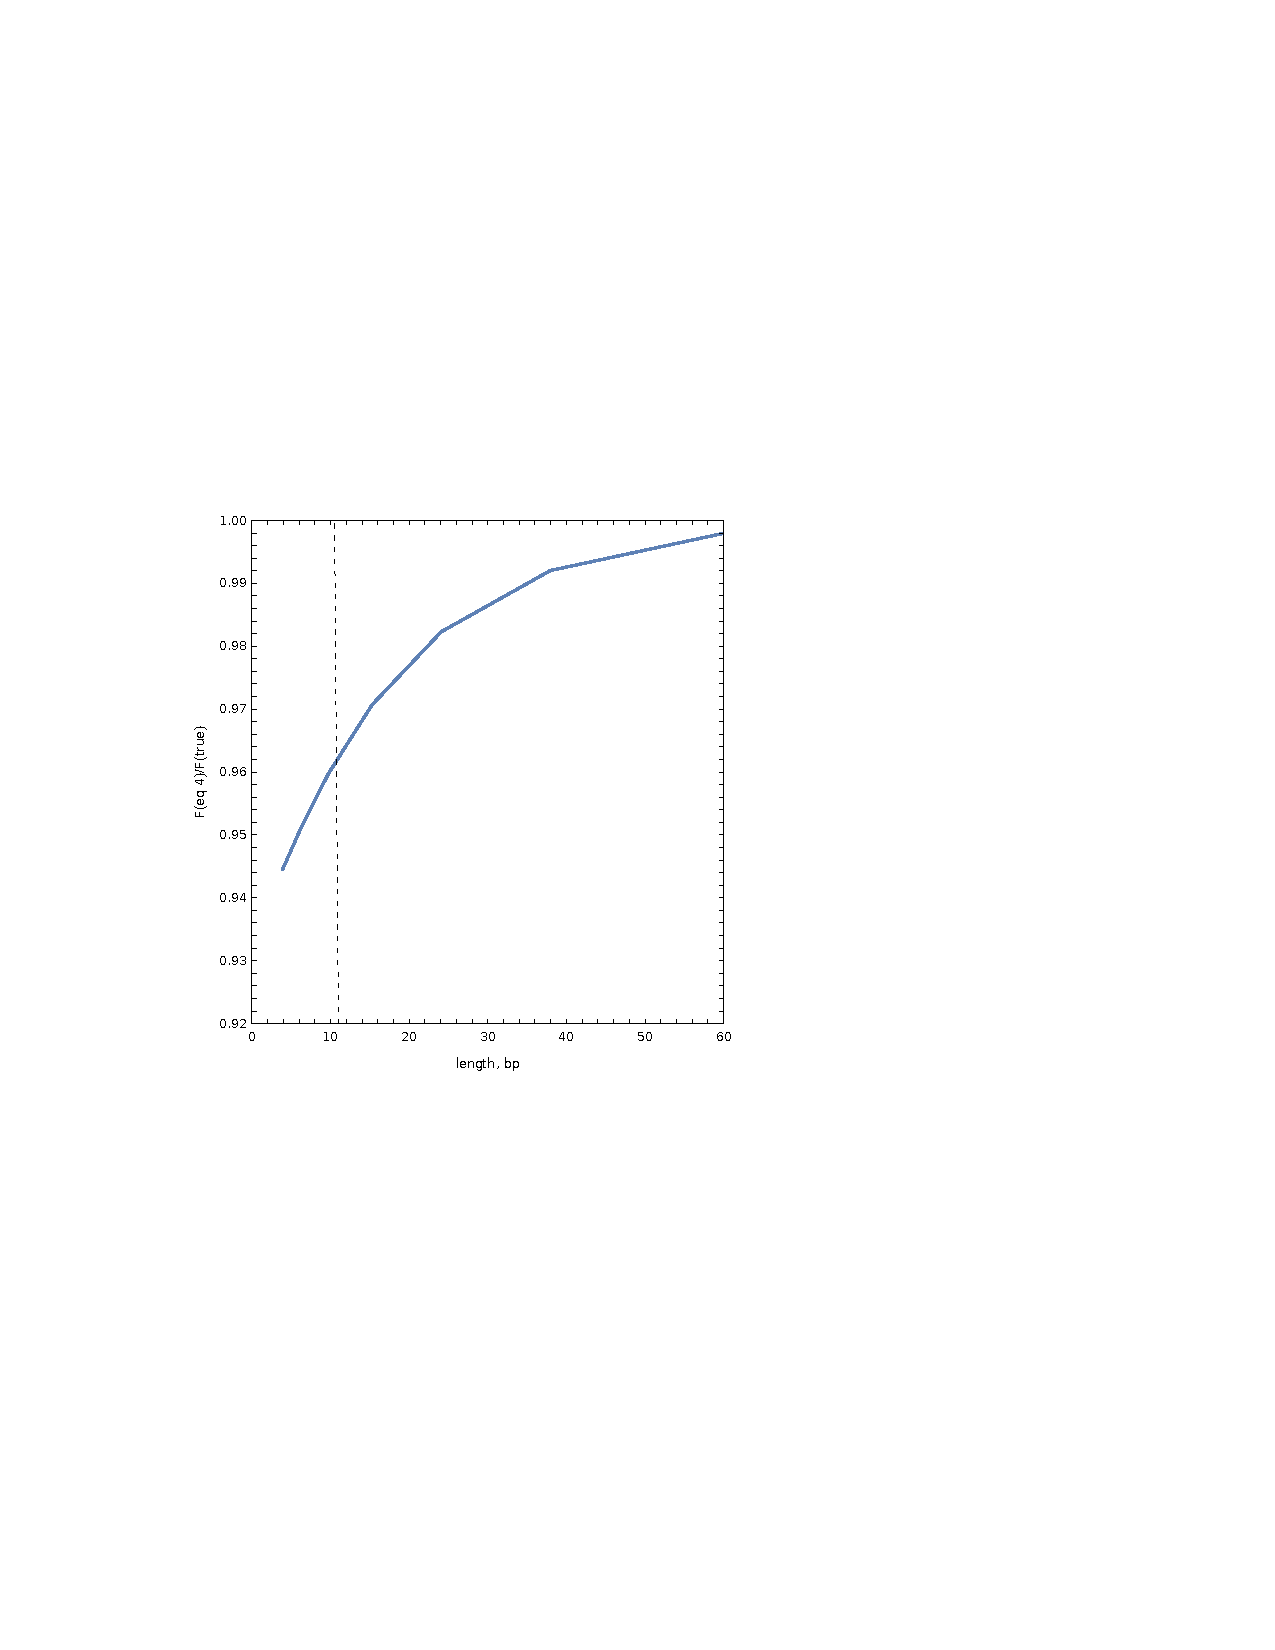
\includegraphics[width=0.5\textwidth]{figs/figure3M12.pdf}
\caption{Recalculation by Mathematica 12.0 of the ratio of the hydrodynamic force on dissimilar spheres using the Kirkwood-Bloomfield approximation relative to that of an exact formulation as a function of lollipop spacer length, for comparison to Figure 3 in the original article.}
\label{figure3}
\end{figure}


%\item Figure 4:
\subsection{Dinucleosome wrapping calculations (original Figure 4)}

This figure presented calculations of the translational diffusion coefficient for different conformations of a dinucleosome as a function of the degree of DNA wrapping for comparison with experimental values.
%The original data for this Figure was calculated in the notebooks ``hydro MS 94/Example 2 1-over-r.nb" and plotted in ``Example 2 dinucleosomes.nb".

Here I again I had to guess that the notebook depended on my library functions. Also, on execution, Mathematica generated a runtime error: ``Set::wrsym: Symbol MonteCarlo is Protected." This resulted from my use of a Boolean variable called ``MonteCarlo", which collided with a Mathematica option name that was defined in version 5.2; renaming the variable to all lowercase solved the problem.

Although the notebook then executed without error, the calculated values reproduced those in the 1995 notebook only to within 4 significant figures, despite the fact that both the new and the 1995 output provided 6 figures. Digging further revealed that after the creation of this figure I had applied a small correction to the average chain statistics in the ``doKirkwood" function in the library s6.1, but which I apparently judged too insignificant to justify re-running the calculations at the time. In support of this hypothesis, I found the earlier version of doKirkwood in my previous version of the library, which I added to s6.1\_repro.nb as ``doKirkwood0", and which produced identical results to those obtained in the 1995 notebook and plotted in Figure 4 of the article (see Table \ref{table}). Note that the difference between the two values with and without the correction is minor and decreases even further as more DNA is wrapped onto the nucleosome (as the length of the linker DNA is correspondingly reduced). The reproduced values are shown in Figure \ref{figure4}.
% (B-form DNA's persistence length is on the order of 150 bp)

\begin{table}[H]
\caption{Dinucleosome sedimentation coefficients in Svedberg units, calculated with and without average distance correction}
\begin{center}
\small
\begin{tabular}{c|c|c}
Superhelical turns & as published & with later correction \\
\hline
1.5	& 1.95652 & 1.96035 \\
1.6	& 2.08147 & 2.08471 \\
1.7	& 2.24511 & 2.2478 \\
1.8	& 2.49574 & 2.4978 \\
1.9	& 2.79165 & 2.79306 \\
2.0	& 3.02864 & 3.02924 \\
\end{tabular}
\normalsize
\end{center}
\label{table}
\end{table}
%%
\begin{figure}[H]
\centering
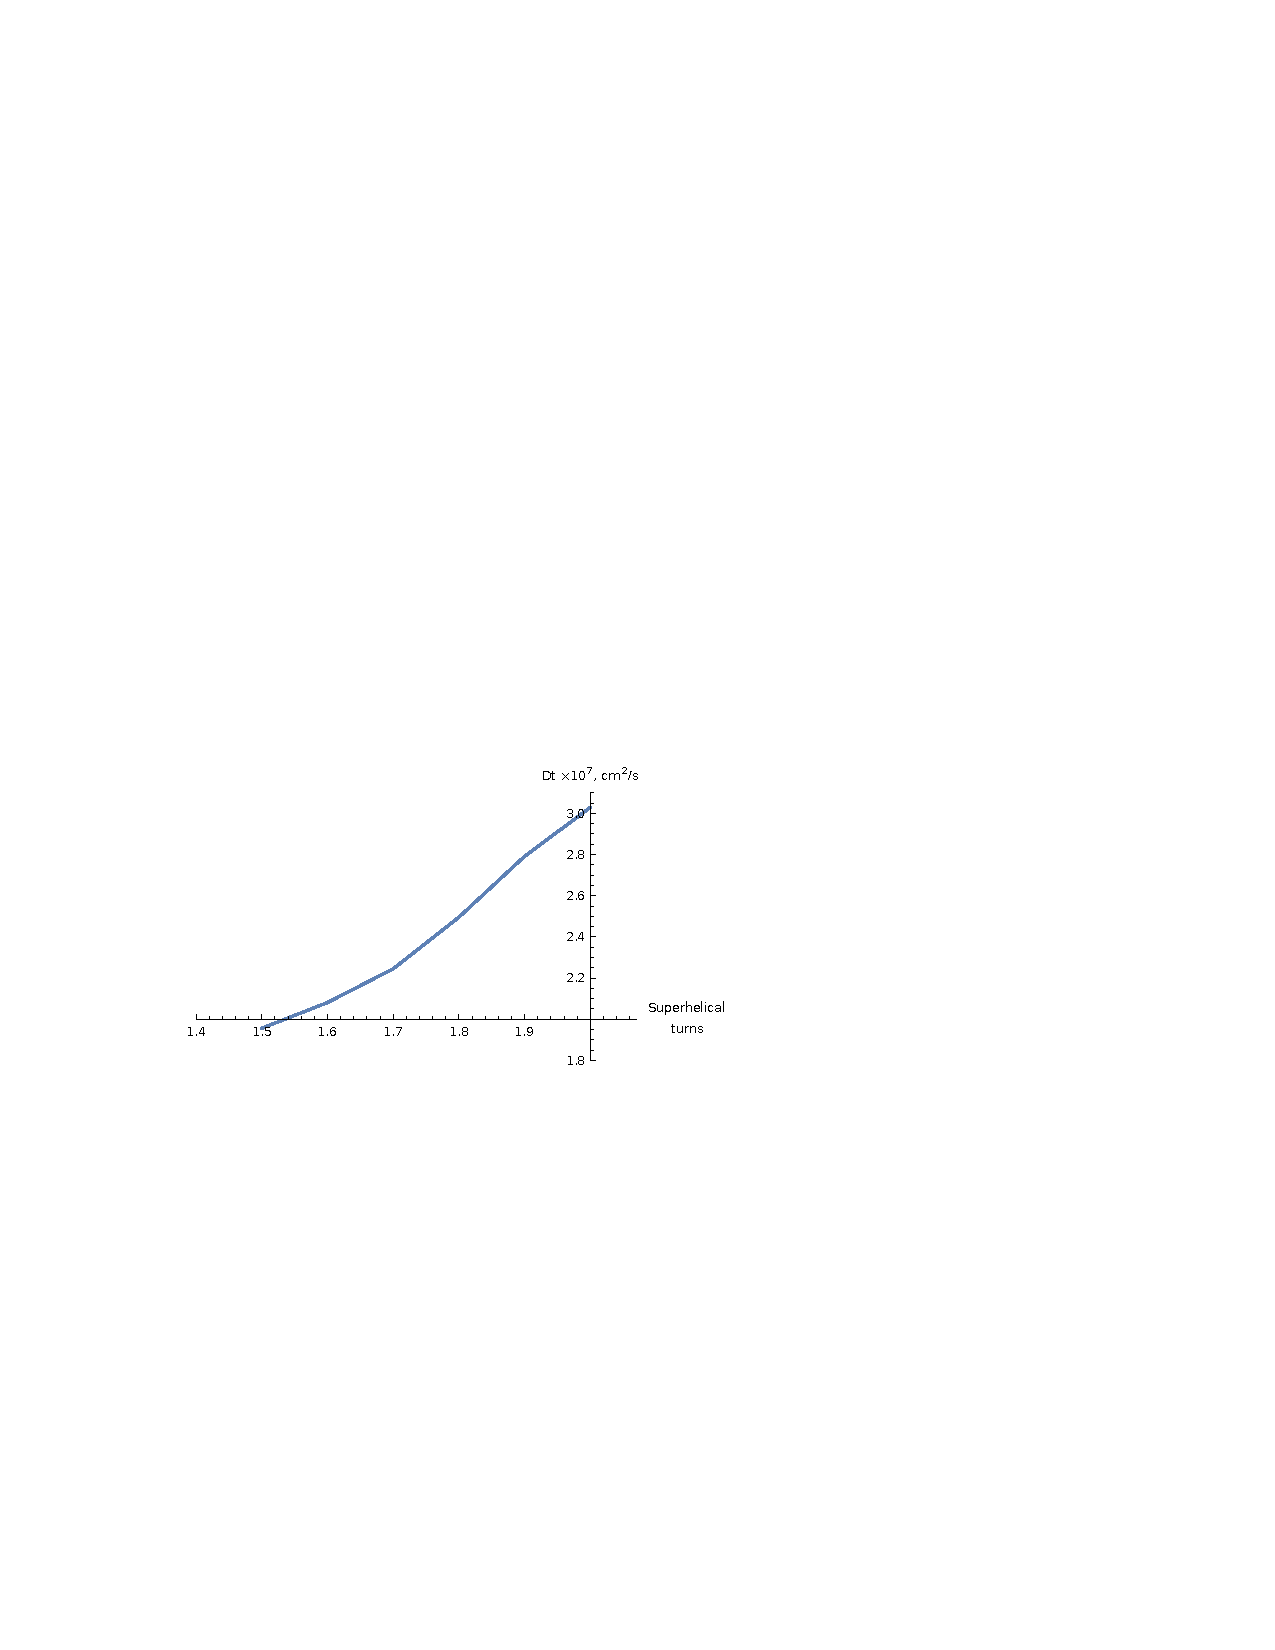
\includegraphics[width=0.5\textwidth]{figs/figure4M12.pdf}
\caption{Recalculation by Mathematica 12.0 of the translational diffusion coefficient for a dinucleosome as a function of the number of superhelical turns, for comparison to Figure 4 of the original article.}
\label{figure4}
\end{figure}

%\item Figure 5 / Table
\subsection{Analysis of compaction intermediates (original Figure 5 and table)}

The article also demonstrated the new approach through the calculation of sedimentation coefficients for all intermediate species in the saturation of a three-site DNA template during progressive compaction by nucleosome formation, which would have been out of reach using existing methods at the time.
%The relevant data for this Figure was calculated in the notebook ``hydro MS 94/Example 3 3x208.nb".
 
This code again depended on functions defined in the library s6.1 as well as a few other generic functions for plotting, which I identified using grep and meta-filedata (here, the file date) to identify the relevant older versions of my general library functions.

In the article, the value for the free DNA template was calculated using an existing method in order to plot the complete sedimentation coefficient distributions at the half-saturation point. However, for some reason only the function which returned the hydrodynamic radius remained. I didn't pursue this particular omission further; in any case the method for calculating the friction properties of the free DNA species alone pre-existed the approach presented in the article.

Scrutinizing my original notebooks revealed another problematic aspect of notebook computing. The function doKirkwood coordinates the calculation of the frictional properties of a given macromolecular species and reports them along with other results obtained by calling additional functions. In the 1995 output, one such derived value was the sedimentation coefficient (s1, the 3rd value in brackets printed for each intermediate species). However, it was not calculated by doKirkwood; only the symbol ``s1" was output, and no numerical value. A likely explanation is that before running the loop I had manually executed the cell defining doKirkwood in my library notebook, but not the cell defining the ``sediment" function (I had not used the ``Get" command to load the separate file). This would explain why the sedimentation coefficients were calculated from the friction coefficients separately, after manually executing the cell defining the ``sediment" function. Of course, no concrete trace of this execution order remains, and this example serves as an example of the pitfalls of ``hidden state" in notebook computing.

Regardless, all friction and sedimentation coefficients calculated for the DNA-protein complexes, together with the bar charts representing the sedimentation coefficient distributions for two possible saturation models, were reproduced exactly as in the Table and Figure 5 of the 1995 article (see Table \ref{tablediff} and Figure \ref{figure5}).

\begin{table}[H]
\small
\caption{Re-calculated nucleosome saturation intermediates for a DNA chain consisting of three 208-bp positioning sequences (20°C)}
\begin{center}
\begin{tabular}{c|c|c}
Species$^a$ & Friction coefficient, $10^{-7}g/s$ & Sedimentation coefficient, S\\
\hline
free DNA$^b$	& —	& 8.1$^b$ \\
\{1\}		& 3.69942 & 9.49818 \\
\{2\}		& 3.44271 & 10.2064 \\
\{3\}		& 3.39772 & 10.3416 \\
\{1,2\}	& 2.86755 & 13.8108 \\
\{1,3\}	& 3.25362 & 12.172 \\
\{2,3\}	&  2.58136& 15.3419 \\
\{1,2,3\}	& 2.15597 & 20.4401 \\
\end{tabular}
\end{center}
$^a$ Species defined by occupied site(s) in chain of sequential sites\\
$^b$ Free DNA species properties were not recalculated.
\normalsize
\label{tablediff}
\end{table}
%
\begin{figure}[H]
\centering
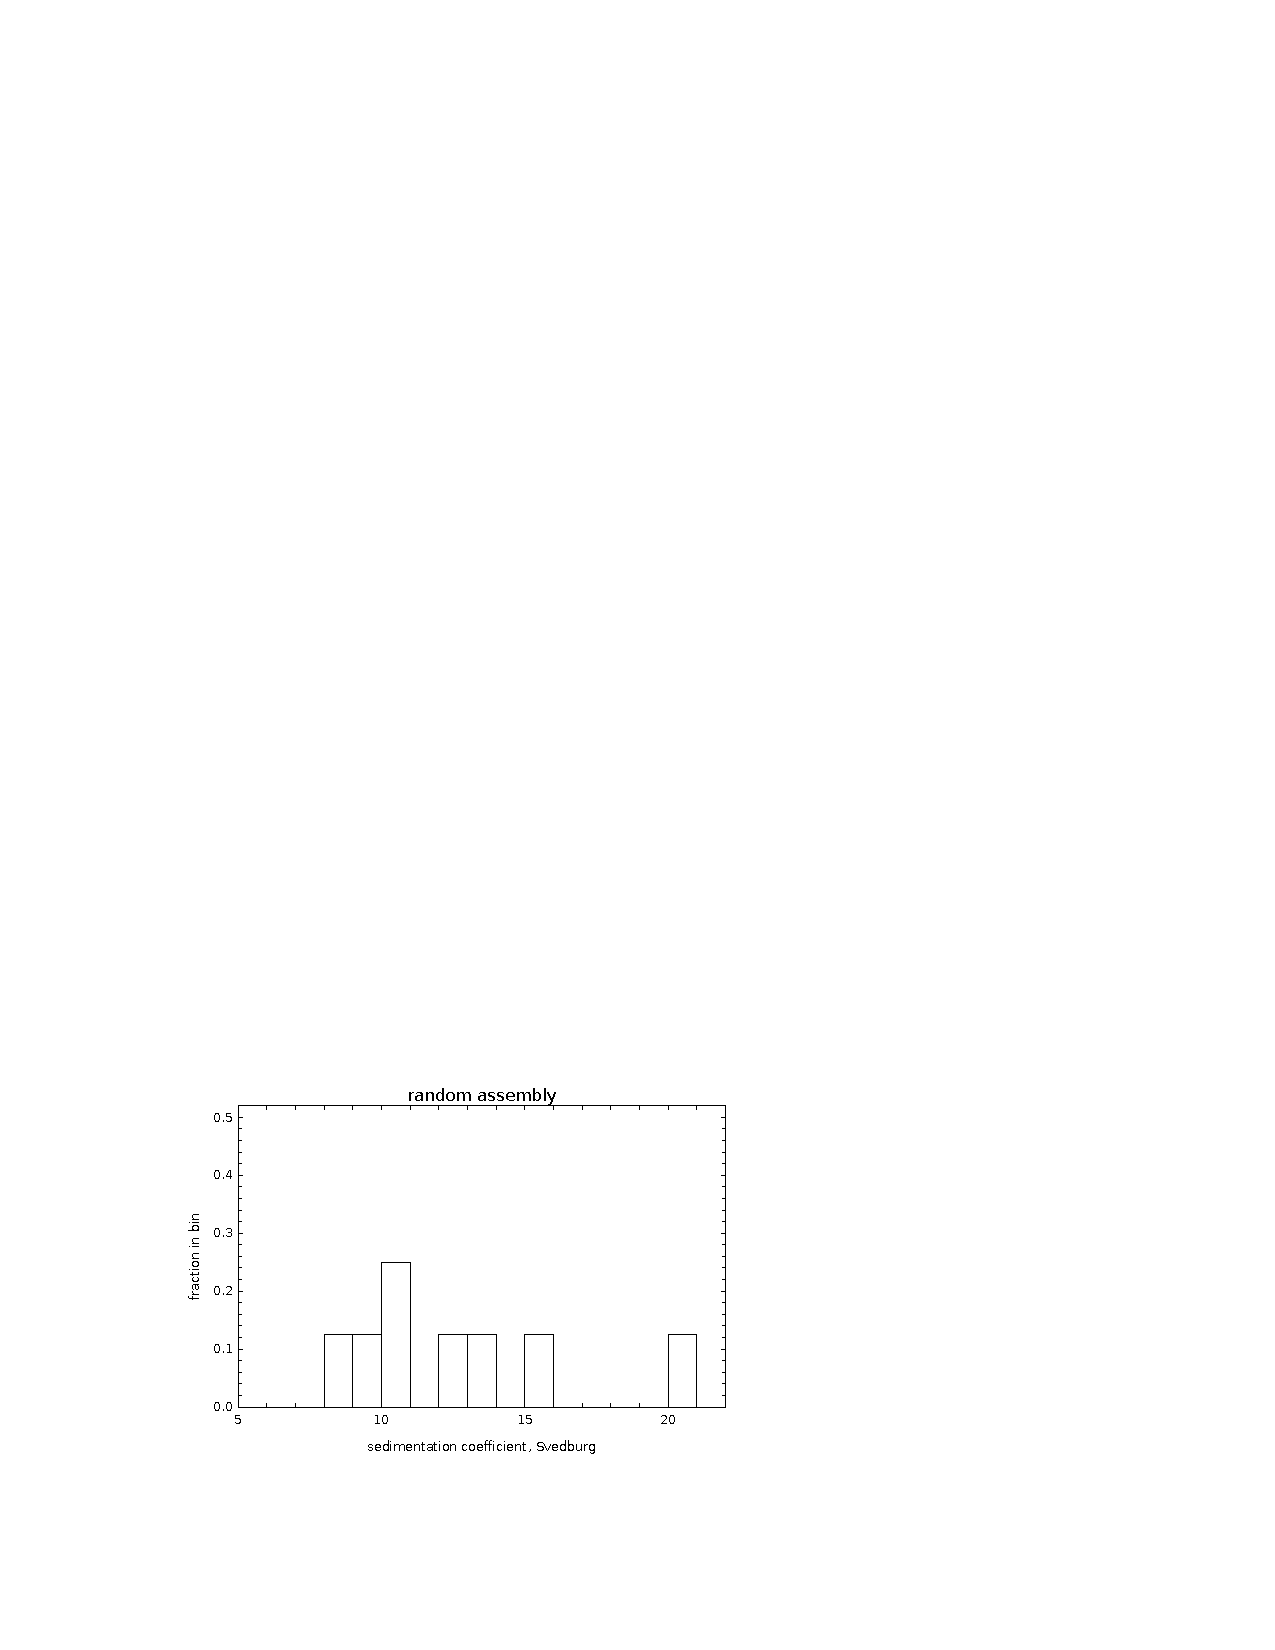
\includegraphics[width=0.45\textwidth]{figs/figure5aM12.pdf}
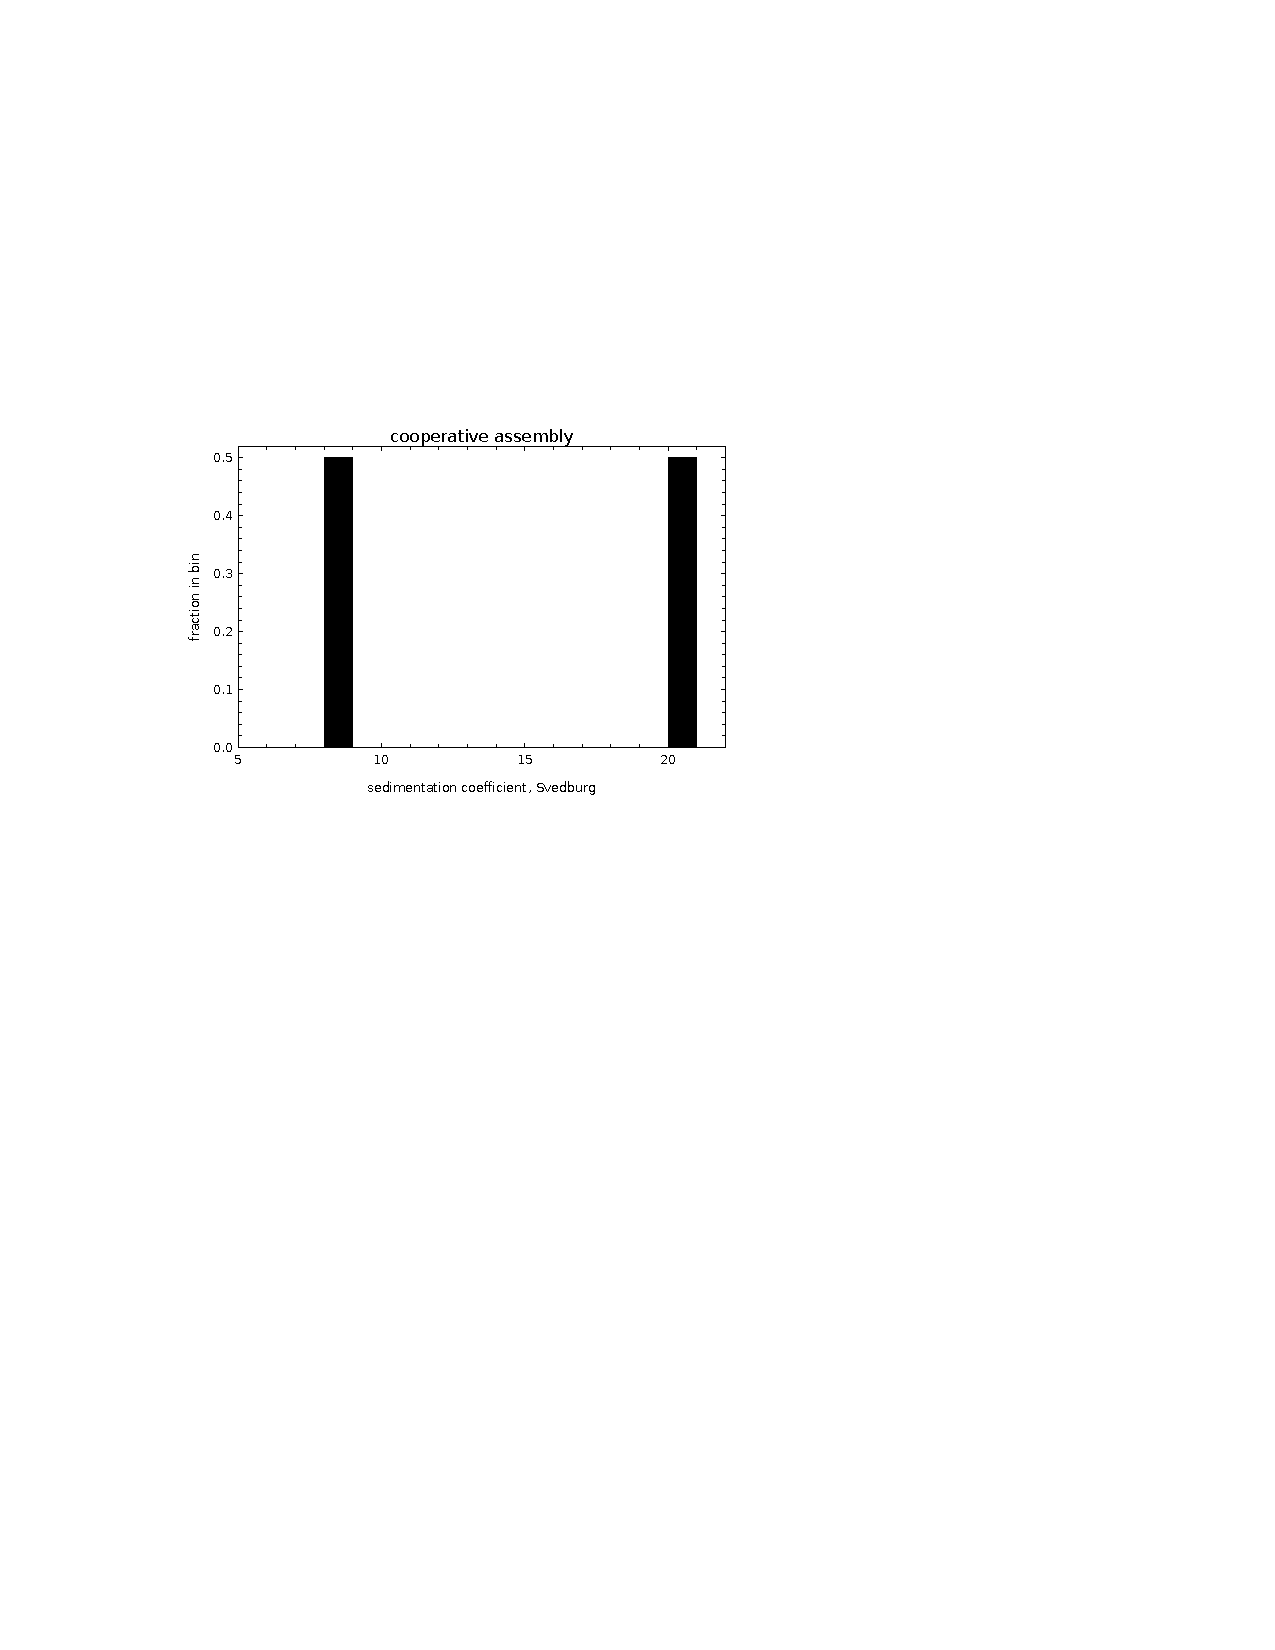
\includegraphics[width=0.45\textwidth]{figs/figure5bM12.pdf}
\caption{Recalculation by Mathematica 12.0 of the distributions of sedimentation coefficients for the compaction of a template consisting of three nucleosome positioning sequences at half saturation, for two different assembly models: random (left) and perfectly cooperative (right), for comparison to Figure 5 of the original article.}
\label{figure5}
\end{figure}
%\end{enumerate}


\section{Conclusions}

I felt fairly confident that I would be able to reproduce the results included in this article on a modern machine, and this was the case. However, it took a bit longer than I had anticipated.

The mid-nineties notebook code, written in Mathematica version 2.2, ran with very few changes on more recent Mathematica versions  (5.2 from 2005 and 12.0 from 2019). The observed incompatibilities were
\begin{itemize}
\item Name collision: a variable name in my code was defined as a reserved word in more recent versions of Mathematica
\item Change in action of trailing semicolon in later versions of Mathematica
\item Plotting option names were changed in more recent versions
\end{itemize}
Only the first involved the calculations directly, and all issues were minor and could be expected in any evolving language.

One might note that a particular consequence of Mathematica's symbolic processing capabilities is that it will not automatically throw an error if a non-numerical result results from a calculation. This is the case if a function has simply not been defined, as was the case in the last example discussed above. Mathematica will happily provide output consisting of the symbolic function name mixed with numerical values for other symbols. This behavior is obviously critical for symbolic manipulations, but it makes it more difficult to identify omitted function definitions.
 
A more significant barrier came from my neglecting to add documentation for the dependencies of the notebook code on functions and definitions made in other notebooks. Mathematica pioneered the use of notebooks on the Macintosh in the 1980's, but it's only been in more recent years that notebook interfaces such as Jupyter have received widespread adoption, (\textit{e.g.}, Rule \textit{et al.} \supercite{Rule2019}). When using notebooks for significant tasks, the problem of dependencies, or more generally, state, can be particularly dogging, as notebooks implicitly encourage state to be established interactively, as opposed to programmatically. Despite being an early proponent, I could already see the madness notebooks could engender, and as a consequence even in the 1990s I made some efforts to organize my code and to perform rudimentary versioning. While incomplete, twenty-five years later this allowed me to reconstruct the dependencies used for this article without too much effort. I only wish I had gone further and taken the time to employ resources such as packages already offered in Mathematica to do so.

A vexing aspect of my 1990's code had nothing to do with Mathematica or notebooks in general: the liberal use of global variables. The notebooks were consistent, but coordinating several notebooks required chasing down each variable in different contexts. This adds a barrier to re-using the code for other applications.

Nevertheless, the calculations presented in the 1995 article could be reproduced, with some effort, in three different 2020 computing environments from the original code. One reason for this is the self-consistency and continuity in the development of Mathematica itself, which began seven years before the target article's publication and continues to this day.

A second type of continuity that might be mentioned is that implied in developing this scientific subject over several years, alternating with other topics, which obliged me to document and modularize my own code (although the result was decidedly far from perfect!). A short-term, one-off project would perhaps have produced a very different result if I had to reproduce it 25 years later. Indeed, while it is clearly in no way optimal, seeing this code running in a modern environment encourages me to continue its development in light of mounting advances both in quantifying chromatin remodelling and in appreciating its biological importance.


\section{Acknowledgements}
Thanks to Wolfram Research for making Mathematica available on the Raspberry Pi platform, which allowed me to test using version 12.0, to the French CNRS program 80|PRIME-2019 (Projet ``DECRYPTOR"), and more generally to the ``Initiative d'Excellence" program from  the French State (Grants ``DYNAMO", ANR-11-LABX-0011, and ``CACSICE", ANR-11-EQPX-0008). Special thanks to Luc Boulesteix, who kindly lent me his Raspberry Pi as one of the test environments.

%\bibliography{}
